\documentclass[english, 11pt, a4paper]{article}
\usepackage{amsmath, amssymb,amsthm}
\usepackage{setspace, natbib}
\usepackage{bm}
\usepackage{threeparttable}
\usepackage{graphicx}
\usepackage{booktabs}
\usepackage{dcolumn}
\usepackage{tabu}
\usepackage{longtable}
\usepackage{float}
\usepackage{caption}
\usepackage{subcaption}
\usepackage[procnames]{listings}
\usepackage{color}
\setlength{\textwidth}{15.5cm} \setlength{\textheight}{22cm}\setlength{\oddsidemargin}{-0.5mm}
\setlength{\parskip}{1ex plus0.5ex minus0.5ex}\setlength{\parindent}{0mm}
\DeclareMathOperator\erfc{erfc}
\usepackage{babel}


\definecolor{keywords}{RGB}{255,0,90}
\definecolor{comments}{RGB}{0,0,113}
\definecolor{red}{RGB}{160,0,0}
\definecolor{green}{RGB}{0,150,0}
 
\lstset{language=Python, 
        basicstyle=\ttfamily\small, 
        keywordstyle=\color{keywords},
        commentstyle=\color{comments},
        stringstyle=\color{red},
        showstringspaces=false,
        identifierstyle=\color{green},
        procnamekeys={def,class}}


\renewcommand{\bibfont}{\footnotesize}
\setlength{\bibsep}{1pt}

\begin{document}

\baselineskip18pt


\title{Order Book Analysis}

\author{Artagan Malsagov}

\date{\today}


\maketitle
%\newpage 
%\tableofcontents

%\section{Introduction}

\section{Data Description}

The data consist of 5 levels of both sides of the order book, for 5 different days.
Each days spans roughly 10 hours worth of data (36 billion micros, see table below)

\begin{table}[H]
    \centering
    \begin{tabular}{lrrrr}
    \toprule
    date & min timestamp & max timestamp & avg bbo mid & avg 5 level order volume \\
    \midrule
    20190610 & 0 & 36000000000 & 10064 & 673 \\
    20190611 & 0 & 36000000000 & 10127 & 866 \\
    20190612 & 0 & 36000000000 & 9999 & 955 \\
    20190613 & 0 & 36000000000 & 10065 & 908 \\
    20190614 & 0 & 35999621354 & 9894 & 797 \\
    \bottomrule
    \end{tabular}
    \caption{Statistics per day of data}
    \label{tab2}
\end{table}


\subsection{Data resampling}
The order book is of the form below:

\begin{table}[H]
    \centering
    \begin{tabular}{crrrr}
    \toprule
    timestamp & bp0 & bq0 & ap0 & aq0 \\
    \midrule
    110 & 10045& 62 & 10055 & 98 \\
    175 & 10065& 46 & 10075 & 42 \\
    220 & 10075& 9 & 10080 & 25 \\
    \bottomrule
    \end{tabular}
    \caption{Subset of the data}
    \label{tab2}
\end{table}

where the timestamps are in microseconds (and there are 4 additional levels of the orderbook).
Plotting a histogram of the frequency of the microsecond timestamps,
we see that the updates aren't uniformly distributed: 

 \begin{figure}[H] 
	\centering
	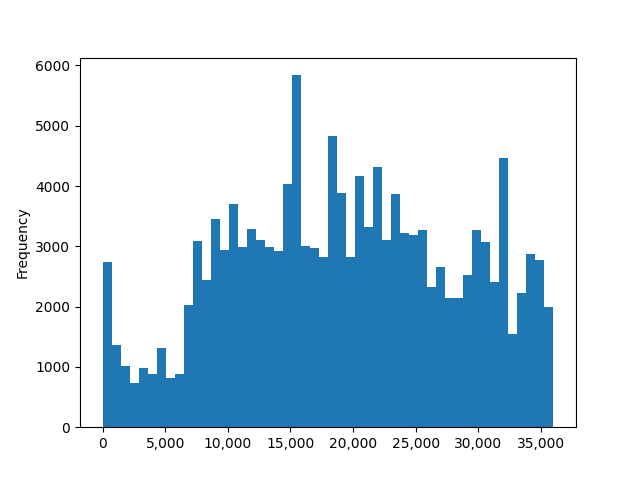
\includegraphics[width=0.90\textwidth]{../data/figures/hist_20190610_timestamps.png}
	\caption{Histogram of order update arrivals for date 20190610}
	\label{fig1}
\end{figure}

For the analysis the data will be resampled. Specifically, a grid will be used with a time interval of
100,000 micros = 100ms. This is done so as to reduce noise of the raw updates at the microsecond
level and thus make signal detection in the data easier. Obviously, this choice of grid size might cause information loss and a more thorough
analysis can be done to optimize, but for practical considerations the 100ms will be used as the
discretization step, since this will allow for quicker data processing and model estimation. 
In practice this means the timestamps will be rounded up to the nearest 100,000 micros.
The reason to round up is to avoid look-ahead bias when using the data as a trade signal, since
rounding down will match an order update with a time-point in the past. In addition, when
discretizing to a grid, there might be an issue when there are no updates available. In that case a
forward interpolation is done by using the last known value of the previous discretization point.

\section{Feature Selection}
\subsection{Target to predict}
For the targets the following metrics were considered:
\begin{itemize}
    \item The simple average mid price:
        \begin{equation}
            P_{mid} = \frac{bp0 + ap0}{2} \label{bbomid}
        \end{equation}
    \item The inverse volume weighted mid price:
        \begin{equation}
            P_{mid}^1 = \frac{bp0\times aq0 + ap0 \times bq0}{bq0 + aq0} \label{invmid1}
        \end{equation}
        This mid has the benefit of taking into account the order imbalance at the top level: if
        the buy order volume is higher, the price will be skewed higher to the ask, and vice-versa
        if the sell order volume is higher.
    \item The inverse volume weighted mid price at the first and second level:
        \begin{equation}
            P_{mid}^2 = \frac{bp0\times aq0 + ap0 \times bq0 + bp1\times aq1 + ap1 \times bq1}{bq0 +
            aq0+bq1+aq1} \label{invmid2}
        \end{equation}
        This mid has the same advantage as the previous one, in addition it also takes into account the
        second layer of the orderbook and thus incorporates more information.
\end{itemize}

For the target the simple average mid (equation \ref{bbomid}) is used rather than one of the two
inverse weighted mids. The reasoning being that the inverse weighted mid prices are already predictors of sorts for the simple average mid. 

Another interesting target would be the mid price change from time $t$ to $t+\delta$ where the $\delta$
is set to a multiple of the discretization step 100ms. The logic being that price moves are what
drives the markets, rather than the absolute price levels. However, to keep things simple, the target
variable to be predicted will be the simple average mid price.

An exploratory analysis of the data is first appropriate. Below are the plots of the mid price and
the inverse weighted mid price $P_{mid}^1$. Looking at the plots there are no weird outliers. Also
clearly the inverse weighted mid price closely tracks the simple average mid price. 
\begin{figure}[H] 
	\centering
	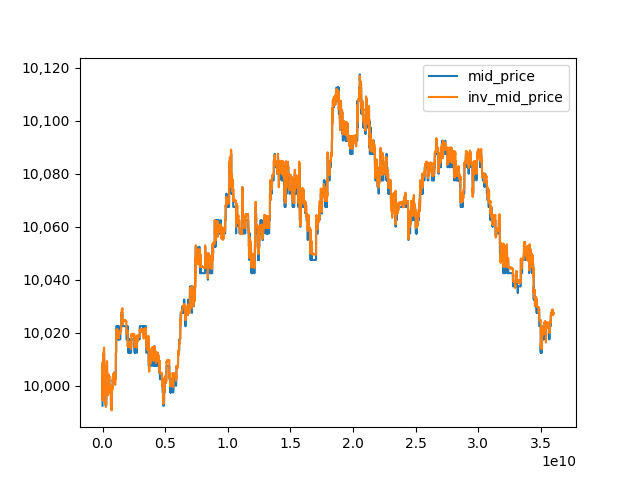
\includegraphics[width=0.70\textwidth]{../data/figures/time_series_20190610_mid_price_inv_mid_price.png}
	\caption{Day 2019-06-10}
	\label{fig2}
\end{figure}

\begin{figure}[H] 
	\centering
	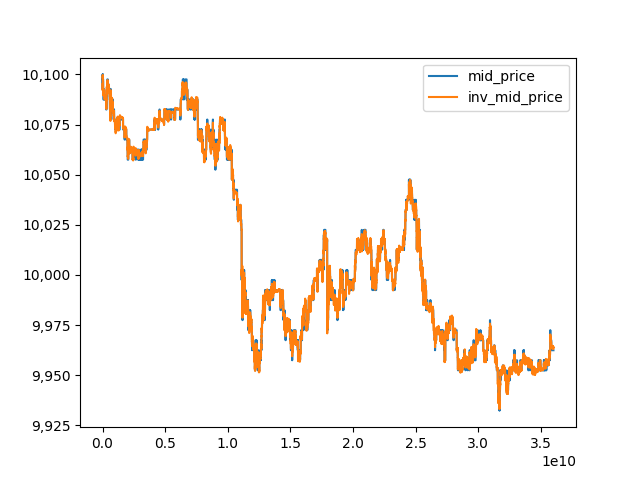
\includegraphics[width=0.70\textwidth]{../data/figures/time_series_20190612_mid_price_inv_mid_price.png}
	\caption{Day 2019-06-12}
	\label{fig3}
\end{figure}

\subsection{Features}
The features below are considered for the analysis:
\begin{itemize}
    \item The bid-offer spread calculated as:
        \begin{equation}
            BOspread = \frac{ap0 - bp0}{P_{mid}}
        \end{equation}
    The intuition of using the spread as a predictor for the change of the mid-price is that if say
    the spread is relatively wide, then the probability of a non-marketable limit order
    arriving whose price is inside the spread is also higher. Whereas if the bid-offer spread was very
    narrow, then the mid-price can only change when one top level side of the order-book is depleted.
    \item Order imbalance at the top level: 
        \begin{equation}
            OI_0 = \frac{bq0}{bq0+aq0} 
        \end{equation}
    The intuition behind this metric is that if the order queue on the bid side is larger than on the
    ask side, the ask side will be depleted sooner and therefore this is predictive of an upward
    price move. Vice-versa a downward move if the ask side queue is larger. This ratio is chosen over a simple subtraction $bq0-aq0$ because the ratio is normalized, which
    reduces bias in the model fitting. Note that if the top level bid size queue is larger than the
    one on the ask side, the ratio will be close to 1. And if the ask side has a much larger
    queue the ratio will be close to 0.
    \item Order imbalance at the second level: same as the above metric, but at the second level of
        the order book:
        \begin{equation}
            OI_1 = \frac{bq1}{bq1+aq1} 
        \end{equation}
    \item Change in $bq0$ relative to the previous time-point on the discretized grid:
        \begin{equation}
            \Delta bq0 = bq0_{t} - bq0_{t-\delta} 
        \end{equation}
        The intuition behind this is that the arrival of a large order on the bid side indicates
        more buying pressure and vice versa when a large buy order is removed by a marketable
        order. Both cases make it likely for the mid price to move.
    \item Change in $aq0$ relative to the previous time-point:
        \begin{equation}
            \Delta aq0 = aq0_{t} - aq0_{t-\delta} 
        \end{equation}
        The intuition behind this is the same as the one for the bid quantity change above. 
    \item Finally the inverse mid price will also be considered as defined in equation
        (\ref{invmid2}). This price is sometimes used as a fair-price in market-making, and the
        analysis will show whether it has any predictive power. Most likely it will be heavily
        correlated with the mid-price.
\end{itemize}



\section{Model Selection}
The model that will be estimated using a Lasso regression is:

\begin{equation}
    P_{mid, t + \delta} = BOspread_{t} + OI_{0, t} + OI_{1,t} + \Delta bq_{0,t} + \Delta aq_{0,t} +
    P_{mid, t}^2 + \beta_0 + \epsilon 
\end{equation}

where $\epsilon$ is the error term and $\beta_0$ is the intercept. For ease of notation, the
coefficients are omitted in the formula above. The forecasted future value of the mid price will be
fixed at $\delta = 100ms$, so one discretization step forward on our grid. Obviously more values can
be tested, but due to time constraints only this value will be used.

Note that the inverse weighted mid price of two layers $P_{mid, t}^2$ will be heavily correlated with $P_{mid}$. 
Hence, the regression will be run twice: with the inverse weighted mid price which will be model 1
and one time without the inverse weighted mid price, model 2:
\begin{equation}
    P_{mid, t + \delta} = BOspread_{t} + OI_{0, t} + OI_{1,t} + \Delta bq_{0,t} + \Delta aq_{0,t} +
    \beta_0 + \epsilon 
\end{equation}


\section{Results}
The model above is estimated using a Lasso regression. Different alphas are experimented with and
the tables report the $R^2$ score and MSE of both the test and train set. The results are given in
the table below:

\begin{table}[H]
  \centering
  \begin{minipage}{.6\textwidth}
    \centering
    \begin{tabular}{lrrrr}
    \toprule
    date & test score & test mse & train score & train mse \\
    \midrule
    20190610 & 0.999716 & 0.233545 & 0.999710 & 0.238649 \\
    20190611 & 0.999766 & 0.129046 & 0.999767 & 0.128842 \\
    20190612 & 0.999935 & 0.141519 & 0.999936 & 0.139918 \\
    20190613 & 0.999639 & 0.161879 & 0.999640 & 0.162173 \\
    20190614 & 0.999900 & 0.225768 & 0.999900 & 0.224700 \\
    \bottomrule
    \end{tabular}
    \caption{Model with $\alpha = 0.04$}
  \end{minipage}
  \begin{minipage}{.6\textwidth}
    \centering
    \begin{tabular}{lrrrr}
    \toprule
    date & test score & test mse & train score & train mse \\
    \midrule
    20190610 & 0.996999 & 2.470786 & 0.997010 & 2.464692 \\
    20190611 & 0.995976 & 2.217756 & 0.995977 & 2.224288 \\
    20190612 & 0.998965 & 2.251413 & 0.998966 & 2.255199 \\
    20190613 & 0.993737 & 2.806957 & 0.993749 & 2.817079 \\
    20190614 & 0.998459 & 3.482738 & 0.998463 & 3.468105 \\
    \bottomrule
    \end{tabular}
    \caption{Model with $\alpha = 1$}
  \end{minipage}
  \begin{minipage}{.6\textwidth}
    \centering
    \begin{tabular}{lrrrr}
    \toprule
    date & test score & test mse & train score & train mse \\
    \midrule
    20190610 & 0.873826 & 103.867544 & 0.873907 & 103.942263 \\
    20190611 & 0.815287 & 101.806958 & 0.815320 & 102.095762 \\
    20190612 & 0.952993 & 102.279769 & 0.952984 & 102.536488 \\
    20190613 & 0.771241 & 102.520754 & 0.771078 & 103.173756 \\
    20190614 & 0.954335 & 103.184173 & 0.954352 & 103.014647 \\
    \bottomrule
    \end{tabular}
    \caption{Model with $\alpha = 10$}
  \end{minipage}
\end{table}


Note that as $\alpha$ is increased, the scores overall go down and the MSEs go up. The scores
overall still remain relatively high though. This is due to the inclusion of  $P_{mid, t}^2$, which is highly correlated with the simple mid
price. Whether $P_{mid, t}^2$ is actually a predictor of the mid price cannot be concluded from
this, since correlation does not mean causation. 

The regression is done again with $P_{mid, t}^2$ omitted, to zoom in on the other variables. See the
tables below. Here it becomes that the other variables don't predict the target variable very well,
which can be observed by the higher MSEs and the lower scores. There might be many issues here, the
choice of discretization step for the grid, the forecast horizon of $\delta = 100ms$, the form of
the target variable: log difference of the mid could have been tested. 


\begin{table}[H]
  \centering
  \begin{minipage}{.6\textwidth}
    \centering
    \begin{tabular}{lrrrr}
    \toprule
    date & test score & test mse & train score & train mse \\
    \midrule
    20190610 & 0.005131 & 818.981603 & 0.005719 & 819.613160 \\
    20190611 & 0.015000 & 542.894661 & 0.014752 & 544.669987 \\
    20190612 & 0.003620 & 2167.974286 & 0.003753 & 2172.710178 \\
    20190613 & 0.074478 & 414.783460 & 0.078335 & 415.389681 \\
    20190614 & 0.186116 & 1839.052605 & 0.187572 & 1833.434636 \\
    \bottomrule
    \end{tabular}
    \caption{Model with $\alpha = 0.04$}
  \end{minipage}
  \begin{minipage}{.6\textwidth}
    \centering
    \begin{tabular}{lrrrr}
    \toprule
    date & test score & test mse & train score & train mse \\
    \midrule
    20190610 & 0.003133 & 820.626689 & 0.003457 & 821.477544 \\
    20190611 & 0.011403 & 544.877094 & 0.011313 & 546.571361 \\
    20190612 & 0.002394 & 2170.641543 & 0.002521 & 2175.395793 \\
    20190613 & 0.068101 & 417.641084 & 0.071400 & 418.515333 \\
    20190614 & 0.184384 & 1842.965925 & 0.185805 & 1837.423822 \\
    \bottomrule
    \end{tabular}
    \caption{Model with $\alpha = 1$}
  \end{minipage}
  \begin{minipage}{.6\textwidth}
    \centering
    \begin{tabular}{lrrrr}
    \toprule
    date & test score & test mse & train score & train mse \\
    \midrule
    20190610 & 0.000000 & 823.205687 & -0.000000 & 824.327841 \\
    20190611 & 0.000000 & 551.162010 & -0.000001 & 552.825785 \\
    20190612 & 0.000000 & 2175.850513 & -0.000002 & 2180.897872 \\
    20190613 & 0.000000 & 448.161418 & -0.000012 & 450.700294 \\
    20190614 & 0.109777 & 2011.549451 & 0.110458 & 2007.460658 \\
    \bottomrule
    \end{tabular}
    \caption{Model with $\alpha = 10$}
    \end{minipage}
\end{table}

Interestingly, date 2019-06-14 has a higher score than the other dates, but also a higher mean
square error. This suggests the model fits the data better for that day, but the predictions still
have a high amount of error. 

The sign of the coefficients is reported in the tables below for $\alpha = 0.04$ for several dates:

\begin{table}[H]
  \centering
  \begin{minipage}{.25\textwidth}
    \centering
      \begin{tabular}{lr}
      \toprule
      feature & coefficient \\
      \midrule
      $BOspread$ & 0.237939 \\
      $OI_0$ & 2.080445 \\
      $OI_1$ & -0.701317 \\
      $\Delta bq_{0}$ & -0.092875 \\
      $\Delta aq_{0}$ & 0.117881 \\
      \bottomrule
      \end{tabular}
  \caption{ $\alpha = 0.04$ and 2019-06-10}
  \end{minipage}
    \hspace{1cm}
  \begin{minipage}{.25\textwidth}
    \centering
  \begin{tabular}{lr}
  \toprule
  feature & coefficient \\
  \midrule
  $BOspread$ & -1.000401 \\
  $OI_0$ & -0.785708 \\
  $OI_1$ & -2.308759 \\
  $\Delta bq_{0}$ & 0.000000 \\
  $\Delta aq_{0}$ & 0.002927 \\
  \bottomrule
  \end{tabular}
  \caption{ $\alpha = 0.04$ and 2019-06-12}
  \end{minipage}
    \hspace{1cm}
  \begin{minipage}{.25\textwidth}
    \centering
    \begin{tabular}{lr}
    \toprule
    feature & coefficient \\
    \midrule
    $BOspread$ & 4.542120 \\
    $OI_0$ & 13.765068 \\
    $OI_1$ & 10.569343 \\
    $\Delta bq_0$ & -0.987877 \\
    $\Delta aq_0$ & 0.441522 \\
    \bottomrule
    \end{tabular}
    \caption{ $\alpha = 0.04$ and 2019-06-14}
  \end{minipage}
\end{table}

\begin{table}[H]
\end{table}

The expectation would be for all coefficients to be positive, since increasing values of the
variables indicate buying pressure and decreasing value indicate selling pressure. However, several
coefficients are negative, however with low absolute value. There was not enough time to include the
statistical significance of these coefficients, however, it is likely that they are not
statistically significant. Furthermore, on date 2019-06-14, the magnitude of two order imbalance
variables ($OI_0$ and $OI_1$) is quite substantial. This is likely related with the test
scores being very high for that date. Further investigation is needed to improve and test for better models. 

%%\section{Conclusion}       

\bibliographystyle{plain}
%\bibliography{report_sci_comp_3}

\end{document}
